\documentclass[11pt]{article}
\usepackage[margin=1in]{geometry}
\usepackage{amsmath,amssymb,booktabs,graphicx,xcolor,hyperref,natbib,multirow,caption,subcaption,lmodern,enumitem}
\hypersetup{colorlinks=true,linkcolor=blue!60!black,citecolor=blue!60!black,urlcolor=blue!60!black}
\captionsetup{font=small,labelfont=bf}
\graphicspath{{figures/}}

% ---- names: change the model / architecture name in one place ----
\newcommand{\model}{QLLM-2}
\newcommand{\arch}{PAM-2}
\newcommand{\archlong}{Phase-Associative Memory, real-valued}
\newcommand{\tpp}{Transformer++}
\newcommand{\mamba}{Mamba-2}
\newcommand{\scione}{SCI-1}
\newcommand{\todo}[1]{\textcolor{red}{[TODO: #1]}}

\title{\textbf{\model: An O(1)-State Mind that Keeps Rules, with Knowledge Kept Outside}\\[4pt]
\large Separating intelligence from knowledge in a constant-memory language model}
\author{Gowrav Vishwakarma \\ \small \texttt{gowravvishwakarma@gmail.com} \\[2pt] \small \todo{co-authors / affiliations}}
\date{Draft of \today}

\begin{document}
\maketitle

\begin{abstract}
A language model carries two different things in its context: \emph{knowledge} (facts, records, text that must be reproduced exactly) and \emph{intelligence} (rules inferred from examples, instructions, the gist of what is going on). Transformers keep both in a KV cache that grows with every token; recurrent state-space models keep both in a fixed vector that fills up. We argue the two should be separated: a constant-size \emph{mind} that holds rules and learning, and an outside \emph{library} that holds knowledge and is read on demand. We present \model, built on \arch{} (\archlong): an attention-free body in which a few layers keep per-head $d\times d$ associative notebooks updated by a gated delta rule, keys and queries are phase-coded by a learned, content-modulated clock that writer and reader layers share, a succession memory at the output head carries copy and induction, and the state resets at document boundaries. Inference is $O(1)$ in memory per token; a 128k-token session is held in 1.15\,MB of state against a 4.9\,GB KV cache.
Our evidence is organised by equal-data tiers with pre-registered bars. In the headline control, three bodies of $\sim$103M parameters are trained on the \emph{identical} 1.0B tokens of a science-and-chat mixture (same code, seed and order): \arch{} applies a rule induced from eight examples across thousands of tokens of unrelated text at 0.52 against 0.15 (\mamba) and 0.07 (\tpp; chance 0.125); holds a rule told once in prose at 0.53 against 0.20 and 0.12; and recalls a fact 8k/16k tokens back, beyond its 4k training length, at 0.53/0.41 against $\le$0.18/0.15. The same pattern holds at two earlier tiers (600M tokens, three seeds; 1.5B tokens). The costs are stated: \mamba{} remains the better pure language model at this size (held-out loss 3.378 vs 3.427 nats), the transformer recalls better inside its window (0.92 vs 0.63 at 2k), and \arch{} trains about $2\times$ slower per token. A 386M-parameter \model{} trained to 8B tokens matches Pythia-410M at 10.5B on HellaSwag/ARC-e/PIQA, reaches 0.88 fact recall at 16k, and shows that the rule skill is \emph{maintained by data}, decaying within 1B tokens when its practice documents are cut and returning with a 1B-token lag. Code, logs, pre-registrations and every number in this paper are in the public repository.
\end{abstract}

\section{Introduction}
\label{sec:intro}

The context of a language model is asked to do two jobs at once. One is \textbf{knowledge}: hold the exact text, the record, the number, so it can be reproduced later. The other is \textbf{intelligence}: notice the rule behind eight examples, keep an instruction given once, carry the gist of a long session, and apply all of that to inputs never seen. The two jobs want different memories. Knowledge wants exact, growing, addressable storage; intelligence wants a compact state that generalises. A transformer \citep{vaswani2017attention} gives both jobs the same growing KV cache, pays for it at every token, and collapses on both past the length it was trained at. A selective state-space model \citep{gu2023mamba,dao2024mamba2} gives both jobs one fixed vector, which stores facts and rules in competition.

This paper takes the separation as a design principle. \textbf{The mind is $O(1)$:} a constant-size state that is the model's own, trained to hold rules, instructions and learning. \textbf{Knowledge lives outside:} in the session text, in tool results, in a library the mind reads on demand. We do not ask the state to be the library; we ask it to be intelligent, and we measure intelligence on what a library cannot provide: rules inferred from examples and applied to unseen cases, rules told once in prose and applied later, and learning that holds beyond the length the model was trained at.

\paragraph{Contributions.}
\begin{enumerate}[leftmargin=1.4em,itemsep=1pt]
\item \textbf{\arch{}}, an attention-free body (\S\ref{sec:arch}) with four parts that together make the state a mind rather than a buffer: a gated delta-rule notebook per head in a sparse subset of layers, a learned content-modulated \emph{clock} that phase-codes keys and queries and is shared by the layers that only read; a \emph{succession (echo) memory} at the output head; and document-boundary reset. The whole runs in $O(1)$ memory per token with a fused training kernel.
\item \textbf{A measurement protocol} for intelligence-vs-knowledge (\S\ref{sec:protocol}): probes for induced rules at distance, told rules held in state (read against a \emph{no-rule twin}, which we show is necessary), recall beyond the trained length, and one-read reach with $O(1)$ query-time operators; all compared within equal-data tiers against \tpp{} and \mamba{} at matched parameters, tokens and data, with bars written before each run.
\item \textbf{Evidence at three equal-data tiers} (\S\ref{sec:results}): \arch{} beats both baselines on rule-carrying and beyond-length recall by wide, pre-registered margins at 600M (three seeds), 1.5B and 1.0B-on-the-product-recipe tokens, while being level on known benchmarks and slightly behind \mamba{} on held-out loss.
\item \textbf{A product-size run and what it taught us} (\S\ref{sec:sci1}, \S\ref{sec:analysis}): \model-386M to 8B tokens; the rule skill is maintained by data, not acquired once; told and induced rules appear to compete for the same state; thinking traces do not help at this size; and the library closes the reach gap at query time (0.91 at 8k).
\item \textbf{The mind + library package} (\S\ref{sec:package}): exact recall at 32k--128k with $\sim$3\,MB held, BABILong single-fact and relation questions carried to 32k with no tuning on the benchmark, and an honest account of what the library does that the mind does not.
\end{enumerate}

\paragraph{Naming.} The first QLLM \citep{vishwakarma2026pam} was complex-valued: tokens lived in phase space and the notebook retrieved by conjugate phase matching. \arch{} is its real-valued successor: the notebook is a real matrix and the \emph{phase} now lives in the rotary coding of keys and queries, driven by a learned clock. One GEMM per projection and no conjugate in the write made a fused kernel possible; the complex head remains in the codebase as a twin.\footnote{The one matched-parameter comparison on record (September 2026, the earlier body: real 101.9M vs complex 100.4M, same loop) found the real body at parity on WikiText-103 at 100M tokens (4.38 vs 4.36 nats) and better on TinyStories ($-0.24$ NLL), though the real arm ran a more conservative recipe, so it is not a clean one-variable test; no matched comparison exists at the body or scale of this paper. Notebook: \texttt{EXPERIMENTS\_SEMPY.md} ledger row 3; log \texttt{logs/v13\_sempty\_wikitext\_real\_fair\_7af42eb\_20260903\_1628.log}.} We keep the family name for continuity and call the model \model.

\section{Related work}
\label{sec:related}
\textbf{Fast weights and the delta rule.} Writing an outer product $v k^\top$ into a matrix state and reading it with a query is the fast-weight programmer \citep{schlag2021linear,katharopoulos2020transformers}; the delta rule erases the old value at a key before writing \citep{yang2024parallelizing}, and Gated DeltaNet adds a scalar forget gate \citep{yang2024gated}. \arch's notebook update (\S\ref{sec:notebook}) is in this family: per-token retention, erase and write gates on a unit-key delta rule. What we add is around it: the clock, the sparse-notebook/shared-read layout, the echo head, the reset, and the recipe and probes that make the state hold rules.
\textbf{Test-time learning and memory modules.} TTT \citep{sun2024ttt} and Titans \citep{behrouz2024titans} update a memory by gradient steps at inference; RWKV \citep{peng2023rwkv} and Griffin \citep{de2024griffin} mix recurrences with local attention; Based \citep{arora2024based} studies the recall--throughput trade-off of linear attention. We take the opposite position on recall: it is the library's job, and the state is judged on rules.
\textbf{Rotary phase.} RoPE \citep{su2024roformer} codes position as a rotation of query and key. Our clock keeps the rotation but makes its speed a learned function of content, accumulated causally, so the notebook's associations carry a learned notion of \emph{when}.
\textbf{Retrieval.} $k$NN-LM \citep{khandelwal2020knnlm} and RETRO \citep{borgeaud2022retro} fetch text into a transformer. Our library is the same idea at the product level with a different division of labour: the fetch delivers knowledge; the state supplies the rule that decides what to do with it.
\textbf{Benchmarks.} BABILong \citep{kuratov2024babilong}, RULER \citep{hsieh2024ruler} and the lm-eval suite \citep{gao2023lmeval}; recurrent-memory transformers \citep{bulatov2022rmt} as the strongest small tuned baselines on BABILong; Pythia \citep{biderman2023pythia} for matched-token reference points.

\section{\arch: the architecture}
\label{sec:arch}
\arch{} is a stack of pre-norm blocks. Every block has a SwiGLU MLP. A sparse subset of blocks (every fourth, from the fourth) also owns a \emph{notebook} layer; every block above the first notebook that has no notebook of its own \emph{reads} the nearest notebook below it with its own query and gate. A succession memory sits between the last block and the tied output embedding. Figure~\ref{fig:arch} gives the whole model; the Appendix gives the backward pass.

\begin{figure}[t]
\centering
\fbox{\begin{minipage}{0.92\linewidth}\small
\textbf{Block $\ell$ (24 blocks in \model-386M):}\quad
$h \leftarrow h + a_\ell\,\mathrm{SwiGLU}(\mathrm{RMSNorm}(h))$ \\
\hspace*{1.2em}if $\ell \in \{3,7,11,15,19,23\}$:\quad $h \leftarrow h + b_\ell\,\mathrm{PAM}_\ell(\mathrm{RMSNorm}(h))$ \hfill \emph{notebook: write + read, $b_\ell$ init 0.1} \\
\hspace*{1.2em}else if $\ell>3$:\quad $h \leftarrow h + \mathrm{READ}_\ell(\mathrm{RMSNorm}(h);\ S^{(\mathrm{below})}, \phi^{(\mathrm{below})})$ \hfill \emph{shared read of the notebook below, zero-init} \\
\textbf{Head:}\quad $\mathrm{lm} = \mathrm{RMSNorm}(W_{\mathrm{head}}\,z) + W_{\mathrm{eo}}\,\mathrm{ECHO}(z,x)$,\quad logits $= \mathrm{lm}\,E^\top$ \hfill \emph{succession memory, zero-init} \\
\textbf{State per token:} 6 notebooks $\times$ 8 heads $\times$ $128{\times}128$ + the echo notebook + one clock per head: $\approx 1.15$\,MB in bf16, independent of length.
\end{minipage}}
\caption{\arch{} at a glance. Only six of 24 blocks hold a notebook; the others read the notebook below them through the writer's own clock. Nothing in the model grows with the sequence.}
\label{fig:arch}
\end{figure}

\subsection{The notebook: a gated delta rule on a $d\times d$ state}
\label{sec:notebook}
For each head with feature size $d$ (128 here) the notebook is a real matrix $S_t\in\mathbb{R}^{d\times d}$. From the block input $u_t$ we project a query, key and value and three scalar gates per head:
\begin{align}
q_t,k_t,v_t &= \mathrm{split}(W_{qkv}u_t),\qquad k_t \leftarrow k_t/\|k_t\|,\\
r_t &= \exp(-\mathrm{softplus}(w_r^\top u_t + \beta)) \in (0,1) \quad\text{(retention; } \beta=-4),\\
e_t &= \min(\sigma(w_e^\top u_t - 3),\,0.95), \qquad \omega_t = \sigma(w_w^\top u_t) \quad\text{(erase, write)},\\
S_t &= r_t\, S_{t-1}\,(I - e_t\,k_t k_t^\top) \;+\; \omega_t\, v_t k_t^\top, \label{eq:delta}\\
y_t &= \mathrm{silu}(w_o^\top u_t)\cdot S_t\,q_t / \sqrt{d}. \label{eq:read}
\end{align}
Equation~\eqref{eq:delta} fades the whole notebook by $r_t$, erases what was stored under the direction $k_t$, then writes the new association. Equation~\eqref{eq:read} reads it with a per-head read-out gate (``N4'' in our ablations). At a document boundary $r_t$ is forced to 0 (\emph{reset at EOS}), so a new document starts from an empty notebook and gradients do not cross document edges. Training runs \eqref{eq:delta}--\eqref{eq:read} in 256-token chunks with a WY-form fused Triton kernel (forward and backward); decoding runs it one token at a time with the same arithmetic, so prefill and decode agree exactly.

\subsection{The clock: content-modulated phase shared by writer and readers}
\label{sec:clock}
Before the write, $q_t$ and $k_t$ are rotated pairwise (as in RoPE) by an angle that is not the position but a \emph{learned cumulative time}:
\begin{equation}
g_t = \exp\!\big(\mathrm{clamp}(w_c^\top u_t,-3,3)\big),\qquad \Phi_t = \sum_{j<t} g_j\, f,\qquad f_i = 10000^{-i/(d/2)},
\end{equation}
with $g_t$ one scalar per head per token. With $w_c=0$ this is exactly RoPE; the model learns to run its clock faster through some tokens and slower through others. Because the rotation is orthogonal and multiplicative, the clock is equivalent to a complex retention $e^{i\theta_t}$ folded into the keys, which is how the phase of the original complex PAM survives in a real model. The clock state $\Phi$ is carried with the notebook, so decoding continues the phase a prefill left off at.

A block that only \emph{reads} rotates its own query by the \emph{writer's} $\Phi_t$, not its own. The query then meets the stored keys in the frame of the layer that wrote them. This is what makes sparse notebooks work: the twelve reader blocks add no state, only a query, a gate and a zero-initialised output projection, and the gradients of every reader flow into the shared notebook.

\subsection{Echo: a succession memory at the head}
\label{sec:echo}
Just before the output embedding, a second delta-rule notebook stores, at the key ``the hidden state one step ago'', the value ``the embedding of the token that came next'':
\begin{equation}
k_t = \mathrm{unit}(W_k z_{t-1}),\qquad v_t = \mathrm{rmsnorm}(E[x_t]),\qquad q_t = W_q z_t,\qquad \mathrm{ECHO}_t = S^{\mathrm{echo}}_t q_t .
\end{equation}
Reading it answers ``what followed the last time the state looked like this'', which is the copy/induction head of a transformer expressed as an $O(1)$ memory. Its output projection is zero-initialised, so the model starts without it and learns to use it.

\subsection{What is new here}
Every piece has a lineage, and we say so: the delta rule \citep{schlag2021linear,yang2024gated}, rotary phase \citep{su2024roformer}, the induction head. The claim is the whole: (i) a learned, content-modulated clock as the phase of an associative notebook, \emph{shared between writing and reading layers} so that six notebooks serve 24 blocks; (ii) a succession memory at the head instead of attention anywhere; (iii) a state that is reset and trained to hold rules (\S\ref{sec:recipe}), and read at query time with two $O(1)$ operators (\S\ref{sec:protocol}); and (iv) the measured consequence: at equal parameters, tokens and data, this state carries induced and told rules and recalls beyond its trained length where both standard families do not (\S\ref{sec:results}). Table~\ref{tab:ablation} lists what each part bought and what we tried and dropped.

\begin{table}[t]
\centering\small
\caption{Component ablations (from the experiment index; each row is a pre-registered keep/drop decision). WikiText-103 perplexity at 102M params; held-out loss (nats) and recall at 600M tokens.}
\label{tab:ablation}
\begin{tabular}{llll}
\toprule
part & what it does & measured effect & verdict \\
\midrule
Chrono clock (\S\ref{sec:clock}) & learned content-modulated phase & WikiText 23.81 $\to$ 23.14 & keep \\
read-out gate & per-head $\mathrm{silu}$ gate on the read & 23.14 $\to$ 22.96 & keep \\
delta rule (\S\ref{sec:notebook}) & erase-before-write, unit keys & 8-way recall micro-bench 0.46 $\to$ 1.00 & keep \\
echo (\S\ref{sec:echo}) & succession memory at the head & holdout 3.541 $\to$ 3.489; WikiText 75.9 $\to$ 71.1; recall 0.34 $\to$ 0.40; PG-19 far gain 2.4$\times$ & keep \\
sparse notebooks & notebooks in 1/4 of the blocks & holdout 3.491 (vs 3.489 dense), recall 0.615, 1.8$\times$ faster & keep \\
shared reads & readers use the notebook below & holdout 3.470 (best LM), recall 0.52, 1.18$\times$ slower than sparse & keep \\
sliding window (128) & local attention in 3 blocks & +0.09 rules at 600M, shrinks with data; hurts the plain body & not in release \\
multi-state / vault & $n$ notebooks per head, one pinned & cost, no decode path & dropped \\
content-routed memories & route writes by key to $S$ notebooks & chance on recall, 4--8$\times$ cost & dropped \\
\bottomrule
\end{tabular}
\end{table}

\section{Training recipe and data}
\label{sec:recipe}
\textbf{Bodies.} Three sizes are used: $\sim$103M parameters (12 blocks, $d_{\text{model}}$ 768, notebooks in blocks 3, 7, 11; the equal-data tiers) and 386M (\model-386M: 24 blocks, $d_{\text{model}}$ 1024, 8 heads $\times$ 128, MLP 3704, notebooks in blocks 3, 7, 11, 15, 19, 23). Baselines are a \tpp{} (RoPE, SwiGLU, RMSNorm) and a \mamba{} of the same parameter count built from the same code base and trained with the same loop; exact counts are in every table.

\textbf{Schedule.} Warmup--stable--decay \citep{hagele2024wsd}, AdamW, peak LR $8\times10^{-4}$, sequence length 4096 (2048 at the small tiers), 65,536 tokens per step at 386M. Runs are resumable from full checkpoints; every continuation is a pre-registered segment with its own hash.

\textbf{Data for \scione{} (the product recipe).} A science-and-chat mixture of filtered public sources: DCLM-baseline and FineWeb-edu for web \citep{li2024dclm,penedo2024fineweb}, arXiv/PubMed/peS2o (Common Pile) for science, Cosmopedia v2, FineMath, SmolTalk chat and multi-turn, tool-calling dialogues (Hermes format), Stack-Edu Python filtered to scientific imports, plus a small synthetic share ($\sim$2.4\% of tokens, $\sim$4\% of loss weight) of \emph{rule documents}: eight-example rule inductions with distractor text between the examples and the query (\texttt{b2s}), long-range recall documents, and prose protocols followed by records (\texttt{proto4k}). Answer tokens in synthetic documents are weighted $100\times$. The mixture is decontaminated against every benchmark reported here with word 13-grams (drops per source in the run header; largest 0.35\%). The first continuation removed thinking traces (\S\ref{sec:think}). All sources are public and the exact weights of each segment are in the repository.

\textbf{The equal-data tiers.} For the architecture claims, each tier trains \arch, \tpp{} and \mamba{} on the \emph{identical} token stream (same sources, weights, seed, order, decontamination and code), so the only difference is the body. The 600M and 1.5B tiers use a general mixture with rule documents; the 1.0B tier uses the \scione{} mixture itself.

\section{Measurement protocol}
\label{sec:protocol}
\textbf{Probes.} \emph{s8 (induced rule at distance):} eight demonstrations of an unseen rule (a letter shift or an affine map over numbers; the families are held out from training), then $L\in\{0,2k,4k,8k\}$ tokens of unrelated held-out text, then a new case; scored as the argmax over 8 candidates (chance 0.125; ``s8 D'' averages the 2k and 4k cells); 400 trials per cell, seeds never used in training. \emph{Told rule:} a protocol stated once in prose (``report every mass in grams to one decimal''), a record thousands of tokens later, then a question; right means value \emph{and} unit/rounding as the rule says; 98--100 documents per cell. \emph{Far needle:} a key--value fact at a distance of 2k--16k tokens, 20-way recall at $L$ beyond the 4k trained length. \emph{Skill pack} and \emph{clk2}: one read of a skill, then $L$ tokens of filler, then a question, with two $O(1)$ query-time operators available to any fixed-state body: \emph{contrast} (the logits of the session minus those of the session without the pack) and \emph{dilation} (reading the notebook with its retention raised to $1/s$ over the filler).

\textbf{The no-rule twin.} A told rule is invisible to the common ``with record vs without record'' contrast: the rule sits in the state in both streams and cancels. Read against the \emph{same session without the rule} (plus the same record), the rule appears (\S\ref{sec:a28}). All told-rule numbers in this paper use the twin read; every day-0 number that used the old read is marked as such in the notebooks.

\textbf{Rules of the comparison.} Claims are made only within a tier (same data, same parameters, same tokens); public models appear only in a reference block and never carry a verdict. Every bar is written before the run (in \texttt{EXPERIMENTS\_SEMPY.md} / \texttt{EXPERIMENTS\_V14.md}), and a failed bar is reported as failed. Cells with fewer than 100 documents are flagged. Mix changes are judged only after two milestones, because effects arrive with a $\sim$1B-token lag (\S\ref{sec:decay}).

\section{Results: the equal-data tiers}
\label{sec:results}

\subsection{The control at the product recipe (1.0B tokens, identical data)}
\begin{figure}[t]\centering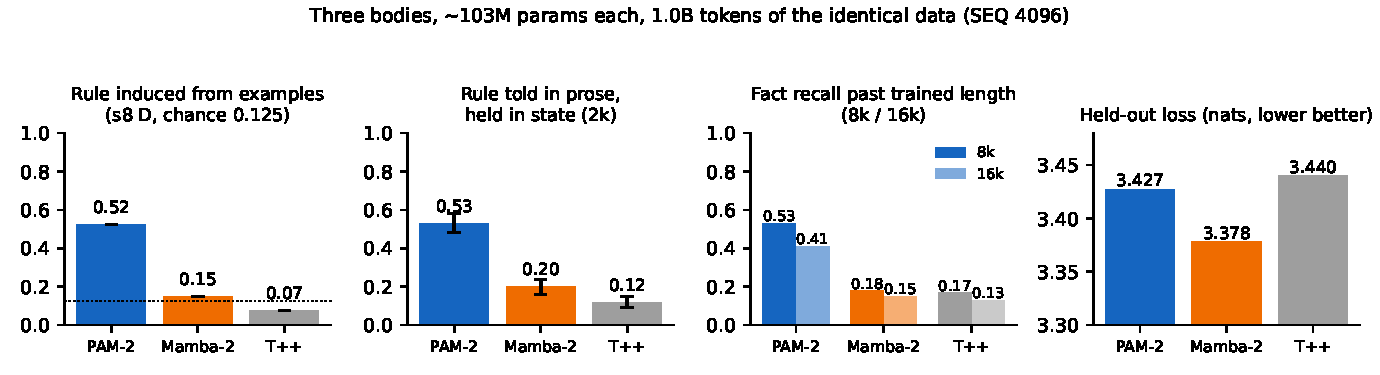
\includegraphics[width=\linewidth]{fig1_control}
\caption{The headline control. Three bodies of $\sim$103M parameters, each trained on the same 1.0B tokens of the \scione{} mixture (same code, seed and order). \arch{} carries an induced rule and a told rule in its state, and recalls beyond its 4k trained length, where both baselines are near chance; \mamba{} is the better pure language model. Error bars: standard error over 98--100 documents.}
\label{fig:control}\end{figure}

\begin{table}[t]\centering\small
\caption{Matched control at the \scione{} recipe: $\sim$103M parameters, 1.0B tokens (0.9B stable + 0.1B decay) of the identical mixture, SEQ 4096, one seed per body. Bars pre-registered before the run; verdicts as written.}
\label{tab:control}
\begin{tabular}{lrrr|l}
\toprule
 & \arch & \mamba & \tpp & bar / verdict \\
\midrule
parameters & 102.88M & 102.61M & 101.92M & \\
induced rule, s8 D (2k+4k) & \textbf{0.523} & 0.149 & 0.074 & $\ge$ best $+0.20$: \textbf{met} ($+0.37$) \\
\quad at $L$ = 0 / 2k / 4k / 8k & .75 / .61 / .43 / .28 & .68 / .18 / .12 / .08 & .36 / .10 / .05 / .05 & \\
told rule in state, 2k (trained wording) & \textbf{0.53 $\pm$ .05} & 0.20 $\pm$ .04 & 0.12 $\pm$ .03 & $\ge$ best $+0.20$: \textbf{met} ($+0.33$) \\
told rule, 2k, held-out wording & 0.12 $\pm$ .03 & 0.06 $\pm$ .02 & 0.05 $\pm$ .02 & $+0.06$: \textbf{not met} \\
told rule, 8k & 0.00 & 0.00 & 0.00 & descriptive \\
far needle 2k / 4k / 8k / 16k & .63 / .63 / \textbf{.53} / \textbf{.41} & .66 / .27 / .18 / .15 & \textbf{.92} / .12 / .17 / .13 & 8k, 16k $\ge$ best $+0.10$: \textbf{met} \\
one read used 8k / 16k later (with operators) & 0.59 / 0.15 & 0.05 / 0.05 & 0.09 / 0.06 & operators are \arch-only; no claim \\
held-out loss (nats) & 3.427 & \textbf{3.378} & 3.440 & $\le$ best $+0.03$: \textbf{not met} ($+0.049$) \\
HellaSwag / ARC-e / PIQA & .282 / .455 / .588 & .284 / .459 / .588 & .281 / .457 / .590 & level \\
training speed on one RTX 4090 (tok/s) & 40k & 113k & 83k & cost \\
\bottomrule
\end{tabular}
\end{table}

Table~\ref{tab:control} and Figure~\ref{fig:control} are the paper's main evidence. With the examples adjacent to the question all three bodies induce the rule (0.75 / 0.68 / 0.36); the difference is \emph{carrying} it across text (Figure~\ref{fig:distance}): at 2k of filler \arch{} keeps 0.61 while \mamba{} falls to 0.18 and \tpp{} to 0.10. The told rule shows the same shape. Beyond the trained length the transformer collapses as expected and the state-space model fades; \arch{} holds 0.41 at $4\times$ its trained length. The costs are equally clear: \mamba{} is 0.049 nats better on held-out text and leads on every web and science source; the transformer is the best reader inside its window; \arch{} trains $2$--$3\times$ slower per token at this size. The held-out-wording cell shows the limit of the told-rule result: at 1B tokens every body holds an unfamiliarly worded rule weakly, and \arch's lead there is small.

\begin{figure}[t]\centering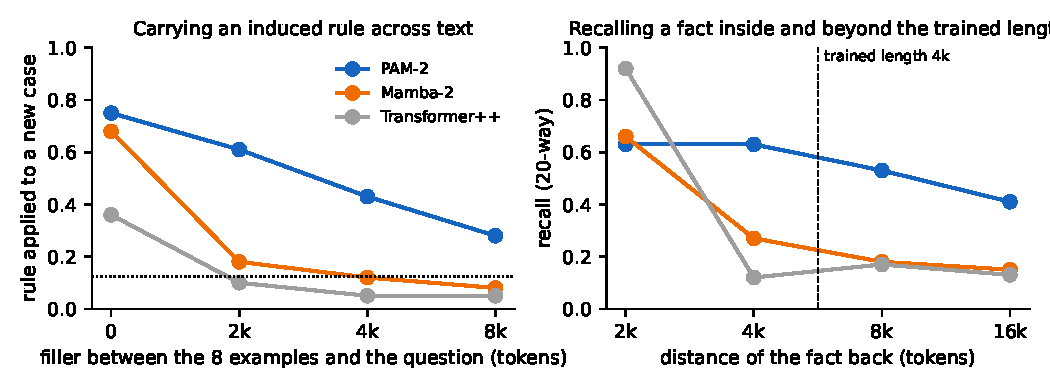
\includegraphics[width=0.9\linewidth]{fig2_distance}
\caption{Where the gap is. Left: a rule induced from eight examples, as the filler between the examples and the question grows. Right: recall of a fact as its distance grows past the 4k trained length. Same three bodies as Table~\ref{tab:control}.}
\label{fig:distance}\end{figure}

\subsection{Two earlier tiers: 600M and 1.5B tokens}
\begin{table}[t]\centering\small
\caption{The equal-data tiers on a general mixture with rule documents ($\sim$102--103M parameters). s8 D at 600M is three seeds for \arch{} (0.645 / 0.691 / 0.741), two for the baselines. ``16nb'' is the plain \arch{} body with a notebook in every block; ``M2'' is the sparse + shared-read body of this paper.}
\label{tab:tiers}
\begin{tabular}{lcc|cccc}
\toprule
 & \multicolumn{2}{c|}{600M tokens} & \multicolumn{4}{c}{1.5B tokens} \\
body & s8 D & holdout & s8 D & rule at $L$=0 & one read used 8k later & holdout \\
\midrule
\arch{} M2 & \textbf{0.69} & 3.480 & \textbf{0.579} & 1.00 & \textbf{0.87} & 3.326 \\
\arch{} 16nb & 0.768 & 3.566 & 0.545 & 1.00 & 0.47 & 3.378 \\
\tpp & 0.134 & 3.557 & 0.047 & 0.53 & 0.29 & 3.359 \\
\mamba & 0.107 & \textbf{3.475} & 0.033 & 0.745 & 0.00 & \textbf{3.303} \\
\bottomrule
\end{tabular}
\end{table}

\begin{figure}[t]\centering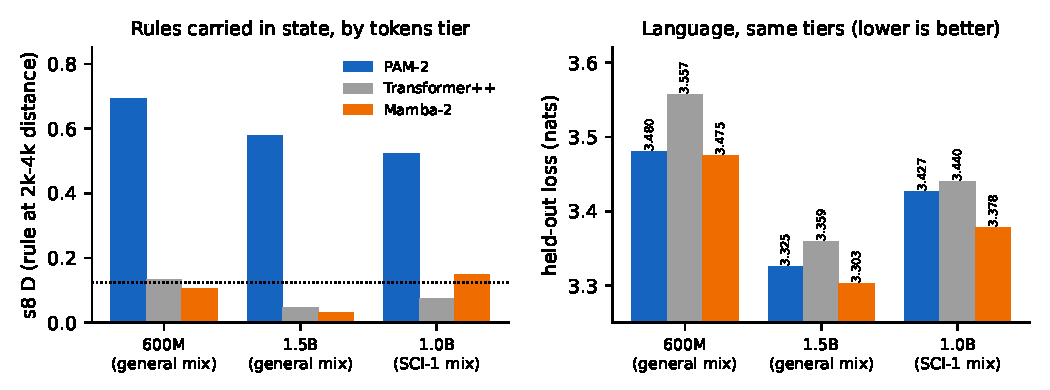
\includegraphics[width=0.9\linewidth]{fig3_tiers}
\caption{Across the equal-data tiers. Left: rules carried in state; right: held-out loss. The ordering never changes: \arch{} on rules, \mamba{} on language, with \arch{} passing the transformer on language at 1.5B and at the \scione{} recipe.}
\label{fig:tiers}\end{figure}

The same ordering appears at 600M and 1.5B tokens (Table~\ref{tab:tiers}, Figure~\ref{fig:tiers}). Two further observations. First, at 1.5B the baselines lose the rule even with no filler at all (0.53 / 0.745 at $L$=0, against 1.00 for both \arch{} bodies): more data made them worse at this skill, not better. Second, \arch's reach with the query-time operators grows with data (one read used 8k later: 0.87 at 1.5B) while the baselines' does not. On a suite of six known multiple-choice benchmarks all three bodies are level at 600M (mean 0.391 / 0.388 / 0.392) and at 3B tokens (0.403 / 0.406 / 0.415); the state's edge is rules, not general knowledge.

\textbf{Rule $\times$ knowledge.} The product case is a rule that lives only in the state applied to a fact that arrives at question time. At 600M tokens, with the fact fetched by the library at 2k, \arch{} answers 0.55 / 0.48 (plain read; 0.61 / 0.62 with the contrast), \tpp{} 0.01 / 0.07, \mamba{} 0.03 / 0.00, and no body answers without the rule (0.00). At 8k \arch{} keeps 0.45 / 0.49. A few-shot ceiling with the rule re-shown at question time gives 0.83--0.92 for \arch{}, 0.30 for \tpp{} and 0.44 for \mamba.

\section{\model-386M: the product-size run}
\label{sec:sci1}
\begin{figure}[t]\centering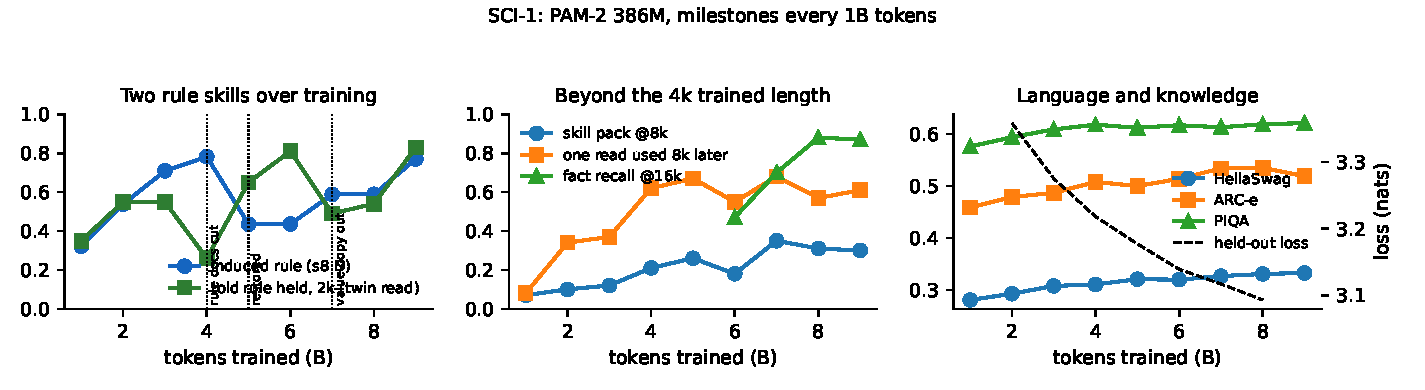
\includegraphics[width=\linewidth]{fig4_sci1}
\caption{\model-386M over 8B tokens, read every 1B. Left: the two rule skills, with the three mix changes marked; the induced skill fell within 1B tokens of its practice documents being cut and returned with a 1B-token lag; the told skill moved the other way. Middle: beyond the 4k trained length, which improved with plain data. Right: language and knowledge improved monotonically.}
\label{fig:sci1}\end{figure}

\model-386M was trained on the \scione{} mixture at sequence length 4096 (0.5B tokens of plain text, then the full mixture), with a full check at every 1B tokens: the probes above, HellaSwag/ARC-e/PIQA, held-out loss, and five fixed generations. Figure~\ref{fig:sci1} shows the first 8B tokens; the run continues to 11.5B at the time of writing \todo{final milestone + decay numbers}.

\textbf{Language and knowledge} improve monotonically: held-out loss 3.358 $\to$ 3.093, ARC-e 0.459 $\to$ 0.535, HellaSwag 0.281 $\to$ 0.331. In a reference block scored with the same harness (fp32; parity with lm-eval to four decimals), \model-386M at 3.0B tokens is level with Pythia-410M \citep{biderman2023pythia} at 10.5B tokens (HS 0.308 vs 0.297, ARC-e 0.487 vs 0.434, PIQA 0.609 vs 0.607) and above it at 4.2B; we attribute this to the filtered data \citep{allal2025smollm2}, not the architecture, and make no claim from it (Figure~\ref{fig:pythia}). On the rule probe Pythia is at chance at every checkpoint including the final 300B (0.03--0.10).

\textbf{Beyond the trained length} improved with plain data: fact recall at 16k rose 0.47 $\to$ 0.88 while training at 4k, and the one-read-at-8k operator from 0.08 to 0.68, with 0.99 recall at 4k and 8k. This is the clause of the thesis that needs no rule documents at all.

\begin{figure}[t]\centering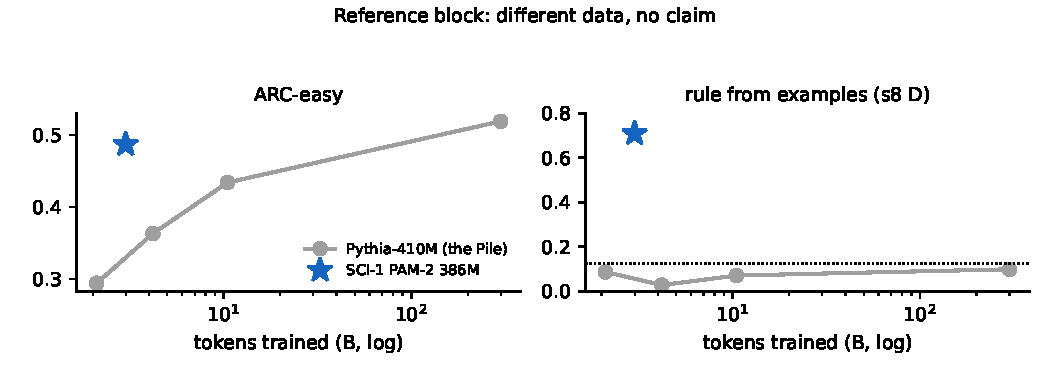
\includegraphics[width=0.85\linewidth]{fig7_pythia}
\caption{Reference block (different data; no claim): \model-386M against Pythia-410M checkpoints on the same harness. Left, ARC-easy; right, the induced-rule probe, where Pythia stays at chance at every token count.}
\label{fig:pythia}\end{figure}

\section{What the product run taught us}
\label{sec:analysis}

\subsection{The rule skill is maintained, not acquired once}
\label{sec:decay}
At 4B tokens the share of rule-induction documents was cut from 1.7\% to 0.5\% of tokens. Within the next 1B tokens the induced-rule score fell from 0.78 to 0.44, while adjacent-example induction (0.96--0.98), recall and one-read reach did not move. Restoring the share to $\sim$1.4\% produced \emph{no} recovery in the first 1B tokens (0.436) and a recovery in the second (0.588), at about the rate of first acquisition. Two conclusions we now treat as rules. Carrying a rule across text in a constant-size state is a practised skill that the data must keep paying for, like a muscle: a product mixture keeps its rule-document share for the life of the run. And a mix change must be judged two milestones later, not one: a 1B-token readout can show nothing yet.

\subsection{Told and induced rules may compete for the state}
Across the same segments the \emph{told} rule moved the other way (Figure~\ref{fig:sci1}, left): 0.26 $\to$ 0.65 $\to$ 0.81 at 2k as the mixture moved weight from induction documents to instruction documents, then back to 0.49 as the induced skill recovered, on an unchanged mixture. In two of three intervals the two skills moved in opposite directions. We state this as a hypothesis from one run: the notebooks are allocated between uses by the data, and a gain in one use can be paid for by the other. If it holds, the architectural answer is per-use protected capacity (a notebook, or a consolidation rule, per use), which we have not yet built. The pre-registered test is running at the time of writing \todo{137,331 readout}.

\subsection{The read was hiding the told rule}
\label{sec:a28}
Our first protocol tests reported that no body applied a told convention (0.00 at every checkpoint). The read was wrong, not the state. The package scored answers as the logits with the record minus the logits without it; a rule held in state sits in both streams and cancels, leaving only the bare value. Read against the \emph{same session without the rule}, \model-386M applies the prose protocol at 0.65 $\pm$ 0.05 at 2k (100 documents; 0.26 at 4B tokens, rising since the first checkpoint), 0.00 under the old read, 0.00 without the rule; beyond 2k it is 0.00--0.10 under every read. The same twin read gives Table~\ref{tab:control}'s told-rule row. The lesson travels: any probe that contrasts a rule-in-state question against a no-record twin undercounts the state. A composed contrast (rule twin plus fact twin in one logit sum) was pre-registered and failed: the fact twin raises the copied value and removes the unit, because one logit sum cannot serve both parts of an answer.

\subsection{The library closes the reach gap at query time}
The mind stores a prose rule but does not carry it past $\sim$2k on its own. The package fixes this without training: it rewrites the prose rule into two worked lines placed next to the question. On 100 documents this reads 0.93 at 2k and 0.91 at 8k (0.72 / 0.68 on the trained wording); the old read gives 0.00. For the unit the library could in principle append the unit itself, so this measures the package path, not the mind's understanding; it is the product behaviour nonetheless.

\subsection{Thinking traces do not help at this size}
\label{sec:think}
\scione{} started with 2.4\% of tokens as \texttt{<think>}-style traces behind a ``Reasoning: on/off'' switch, with pre-registered tripwires. At 2B and 4B tokens accuracy on GSM8K test with thinking on was 0.02--0.055 against 0.03--0.04 off, and 24--47\% of ``off'' answers leaked a trace. Re-run with four times the generation budget, 173 of 200 traces finish and reach an answer; the failures are reasoning errors (invented quantities, wrong setup), not truncation. The source was removed at the first continuation and the switch dropped from the chat template; \model{} answers directly. A plain-text worked-solution source (no tags, no switch) is being tested as a long-span trainer \todo{cont4 readout}.

\section{The mind + library package}
\label{sec:package}
\begin{figure}[t]\centering
\begin{subfigure}[t]{0.42\linewidth}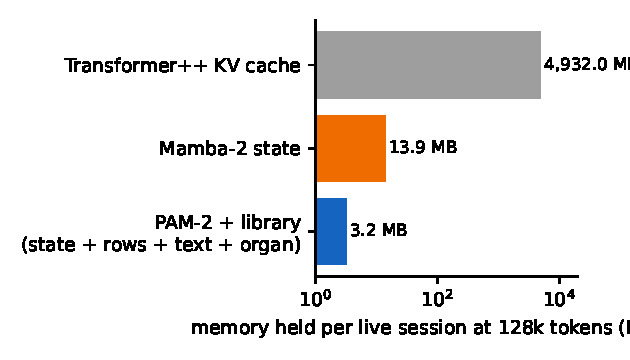
\includegraphics[width=\linewidth]{fig5_memory}\caption{Memory per live session at 128k tokens.}\end{subfigure}\hfill
\begin{subfigure}[t]{0.56\linewidth}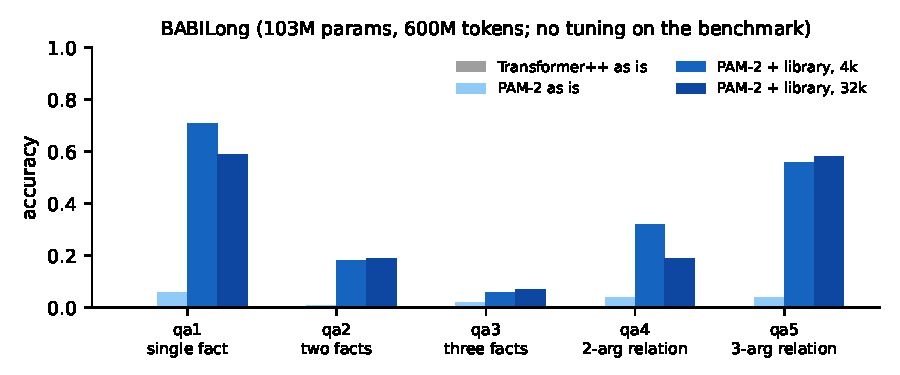
\includegraphics[width=\linewidth]{fig6_babilong}\caption{BABILong qa1--qa5, 100 documents per cell.}\end{subfigure}
\caption{The package at 103M parameters / 600M tokens. (a) The state is 1.15\,MB; with rows, text and the exact-text organ the whole package holds $\sim$3\,MB where a transformer's KV cache holds 4.9\,GB. (b) As is, no body reads BABILong beyond 0k; the package carries single-fact and relation questions to 32k, while two- and three-fact composition stays below 0.20 for every column.}
\label{fig:package}\end{figure}

The library is three parts outside the layers: the session text with an exact-text organ (an $n$-gram index), a row store of fetched facts, and a planner that rewrites and re-reads. Its recall is model-free and we report it as such: needle, 8-needle, latest-wins and two-hop are 1.00 (20-way) at 32k and 128k through the organ for every body, against 0.04--0.14 for any body as is. What belongs to the mind is the constant cost while the session is held (Figure~\ref{fig:package}a), the rule that decides what to do with a fetched fact (\S\ref{sec:results}), and its own-state keys where words differ (synonym keys 0.575 vs 0.35 for a MiniLM index; natural questions 0.775 vs 0.525 for BM25, on the trained template). Two honest lines: a transformer given the same library and a cold read reads single facts as well and multi-field records better (0.90 vs 0.45 for both fixed-state bodies), and the composition of several facts (BABILong qa2/qa3, story order) is unsolved by any body at this size (Figure~\ref{fig:package}b). The strongest small tuned baselines on BABILong (ARMT-137M 97.8\%, fine-tuned Mamba-130M 97.7\%) train on the task; our column is ``as is, no tuning'', and is reported as a reference, not a race.

\section{Limitations}
\begin{itemize}[leftmargin=1.4em,itemsep=1pt]
\item \textbf{Language.} \mamba{} is the better pure language model at every tier we ran (0.02--0.05 nats); \arch{} passes the transformer at 1.5B and at the \scione{} recipe but not \mamba. Closing this gap is the main open problem for the body.
\item \textbf{Seeds.} The 1.0B control and the 1.5B tier are one seed per body; the 600M tier has three \arch{} seeds. A second seed of the control is the next experiment.
\item \textbf{Told rules.} The edge holds on the trained wording; on a held-out wording at 2k it is +0.06 and not significant, and no body carries a told rule to 8k alone. Reach past $\sim$2k for told rules, and past 8k for induced rules, is the library's job today.
\item \textbf{Formats.} The mind generalises values and keys, not formats: reworded questions collapse cold reads for every body at 103M, and the package answers them on natural keys.
\item \textbf{Composition and arithmetic.} Multi-fact composition is unsolved at this size; rounding and unit conversion belong to a code tool, not the state.
\item \textbf{Cost.} Training is $2$--$3\times$ slower per token than the baselines at 103M on one GPU; inference memory is constant.
\item \textbf{Scale.} The largest body here is 386M parameters at 11.5B tokens. Nothing in this paper is evidence about billion-parameter models.
\end{itemize}

\section{Conclusion}
We set out to build a model whose state is a mind rather than a buffer, and to keep knowledge outside it. The evidence, organised in equal-data tiers with bars written in advance, says the state of \arch{} does what we asked of it: it carries rules it induced and rules it was told across thousands of tokens of other text, and it recalls beyond the length it was trained at, where a transformer and a state-space model of the same size trained on the same tokens do not. The same evidence says what it does not do: it is not the best language model at this size, it does not out-read a transformer inside the transformer's window, and it holds a skill only as long as the data keeps training it. We think that trade is the right one to make and the right one to study, because it is the half of the problem that a library cannot solve.

\paragraph{Reproducibility.} Code, every log named by run hash and date, the pre-registrations and verdicts (\texttt{EXPERIMENTS\_SEMPY.md}, \texttt{EXPERIMENTS\_V14.md}), the experiment lineage tree, and the file of numbers this paper is drawn from (\texttt{v16/paper/data/numbers.json}) are in the repository \todo{public URL}; model weights on Hugging Face \todo{release tag}.

\bibliographystyle{plainnat}
\bibliography{refs}

\appendix
\section{Forward and backward pass of a notebook head}
\label{app:bwd}
Write $A_t = r_t(I - e_t k_t k_t^\top)$ (symmetric), so $S_t = S_{t-1}A_t + \omega_t v_t k_t^\top$ and $y_t = c_t\, S_t q_t/\sqrt d$ with $c_t$ the read-out gate. The backward pass runs in reverse time with one carried $d\times d$ adjoint $\bar S$:
\begin{enumerate}[leftmargin=1.6em,itemsep=1pt]
\item $\bar S \gets 0$; for $t = T,\dots,1$:
\item $\bar S \mathrel{+}= c_t\,\bar y_t q_t^\top/\sqrt d \;+\; \sum_{\text{readers}} \bar y'_t q'^\top_t/\sqrt d$ \hfill (readers' gradients flow into the shared notebook)
\item $\bar q_t = c_t S_t^\top \bar y_t/\sqrt d,\qquad \bar c_t = \bar y_t\cdot(S_t q_t)/\sqrt d$
\item $\bar v_t = \omega_t \bar S k_t,\qquad \bar\omega_t = v_t^\top \bar S k_t,\qquad \bar A = S_{t-1}^\top \bar S$
\item $\bar r_t = \langle \bar A,\, I - e_t k_t k_t^\top\rangle,\qquad \bar e_t = -r_t\, k_t^\top \bar A k_t$
\item $\bar k_t = \omega_t \bar S^\top v_t - r_t e_t(\bar A + \bar A^\top)k_t$, then through the unit-norm and the rotation (orthogonal)
\item $\bar S \gets \bar S A_t$ \hfill ($A_t = 0$ at a document boundary: gradients stop at the edge)
\end{enumerate}
Per chunk of 256 tokens the same recursion is a WY-form kernel (one batched solve and one scan per layer).
The clock's gradient follows from $\Phi_t = \sum_{j<t} g_j f$ by a reverse cumulative sum. All other parts (SwiGLU, RMSNorm, linear layers, tied embedding, cross-entropy) are standard.

\section{Run table}
\label{app:runs}
\small
\begin{tabular}{lll}
\toprule
run & what & hash / log \\
\midrule
ctl & matched control, 3 bodies, 1.0B, \scione{} mix & code \texttt{caa4da9}, result \texttt{f0a4695}, \texttt{logs/ctl/} \\
A28 / A28b & told rule, twin read; held-out wording & \texttt{be66f2d}, \texttt{a69cafa}; \texttt{logs/v14\_a28\_*} \\
A29 / A30 & query-time rewrite; composed contrast & \texttt{EXPERIMENTS\_V14} \\
t15 & 1.5B tier, 4 bodies & Mind \texttt{9616861}; t15pam\_m2 verdict \\
b2p2 / tfc1b / mbs2b & 600M tier (3 \arch{} seeds) & \texttt{EXPERIMENTS\_SEMPY}, kb1 \texttt{ccf187c} \\
\scione{} & 386M, segments \texttt{59c3cf5} $\to$ \texttt{59d098d} $\to$ \texttt{e61cd92} $\to$ \texttt{449e320} $\to$ \texttt{8284510} & \texttt{logs/sci1/}, \texttt{logs/diag/}, \texttt{logs/learning\_probes/} \\
Pythia reference & same harness, fp32 & \texttt{78c98e6}, \texttt{logs/sci1ref/} \\
BABILong & package v0, 103M / 600M & \texttt{773d751}, \texttt{logs/v16\_babilong\_*} \\
\bottomrule
\end{tabular}
\end{document}
